\documentclass{response}

\title{Modelling the high-voltage grid using open data for Europe and beyond}
\authors{Bobby Xiong*, Davide Fioriti, Fabian Neumann, Iegor Riepin, Tom Brown\\\footnotesize *corresponding author (\href{mailto:xiong@tu-berlin.de}{xiong@tu-berlin.de})} 
\journal{Scientific Data --- Nature}
\iteration{1}
\date{\today}
 
\bibliographystyle{elsarticle-num}

\usepackage{libertinust1math}
\renewcommand{\ttdefault}{\sfdefault}
\usepackage[nameinlink,sort&compress,capitalise,noabbrev]{cleveref}
\usepackage{lipsum}
\usepackage{hyperref}

\begin{document} 

\maketitle 

We thank the reviewers for their constructive comments and acknowledge the time
and effort they have spent in assessing our work. We have revised the paper
based on the feedback from the reviewers and hope that we can adequately address
their primary concerns.

To follow the revisions made, we have highlighted differences compared with the
previous submitted version of the paper in {\color{blue}{blue}} and
{\color{red}{red}} text in an attached file. Figure numbers in this response letter
refer to the numbering in the revised version of the manuscript.

\section*{General comments by the authors}
With the revision and following your suggestions, we have made various improvements both in the manuscript and the dataset. In the following, we would like to highlight a few, before diving into our individual responses to the editor's and reviewers' comments:
\begin{itemize}
    \item We have added an elaborate description of the dataset, its files, contents, properties and units in the Data Records section. This will help users understand the dataset and facilitate its reuse also outside the PyPSA-Eur model and PyPSA framework.
    \item We have improved the clustering algorithm to allow for a more detailed representation of the grid. The radius for clustering has been reduced to 500 meters, which allows for a much more detailed representation of the grid. Note that with this change, the number of grid components has changed, accordingly. Note that a tolerance of 500 meters is still needed to deal with transmission lines that split into their sub-circuits before reaching a substation they are connecting to (e.g. a double-circuit line splitting into two single-circuit lines --- in many cases, these are mapped out on OpenStreetMap as well). We have updated the manuscript to reflect this change. 
    \item With the improvement in the clustering algorithm, we have re-run our analyses and updated our findings. Exact numbers have changed minimally and overall conclusions remain the same.
    \item The dataset has been updated to include all technical parameters of the grid components which were previously mapped in PyPSA. This allows for the standalone use of the dataset without the need for the PyPSA-Eur model. Furthermore we have added an interactive map to allow for the visual exploration of the dataset.
    \item Remarks regarding the data: We have now added Kosovo (XK) and Moldova (MD) as individual countries in the dataset. Furthermore, between the initial submission and the revised manuscript, a new 600 MW HVDC interconnector, Shetland HVDC Link (\href{https://www.ssen-transmission.co.uk/projects/project-map/shetland}{https://www.ssen-transmission.co.uk/projects/project-map/shetland}) has been commissioned, which is now already part of version 0.6 of the dataset on Zenodo \cite{xiongPrebuiltElectricityNetwork2024}. This shows how fast real changes can be included in the dataset obtained through our presented workflow.
    \item We elaborate on all the remaining editor's and reviewers' comments in the following sections below. 
\end{itemize}

\section*{Editor comments}

\EC Please provide an additional copy of your manuscript file under 20 MB as a \textit{Related Manuscript File} in your next submission for internal use.

\AR With the submission of the revised manuscript, we have included a copy of the manuscript file under 20 MB as a \textit{Related Manuscript File} for internal use, as requested.

\EC A data descriptor provides a description of a static dataset, rather than any novel methods or computational validation schemes. Please edit the text of your abstract to focus more on the dataset that you have generated, rather than a method for constructing the dataset.

\AR Thank you for your feedback and for helping us to improve the clarity and focus of our manuscript. We have revised the abstract to highlight the dataset itself that we have generated, rather than the methodology for its construction.

\EC Because at least some of your data looks to originate from third parties, please check the following and confirm/state what has been done in your \textit{response to reviewers} document:
\begin{enumerate}
    \item All sources are clearly described in either the main text. For general mentions of services, databases, or other platforms, please name the resource in the main text and provide a URL in ()s. Instructions should be sufficient for the exact input data to be retrieved, so please provide specific links, accession numbers, or the exact search term/query when discussing any data from general databases. For specific datasets downloaded from repositories, or other items with formal metadata, please use a full citation in the reference list containing the relevant DOI. Note this should be the dataset, rather than any relevant publication, however these should be cited as well if required, or if the data was newly extracted from a document.
    \item Confirm all the sources are openly available --- i.e. your re-use or re-distribution is compliant with the terms and conditions/licenses for data sharing. If you cannot see a fully open licence at the source please check with the data provider. Please note it is your legal responsibility to ensure all data have been used or re-distributed appropriately and we cannot support publication of descriptions of data obtained or re-shared without this check.
\end{enumerate}

\AR Thank you for the detailed review and guidance on data sourcing and citation requirements. We have taken the following steps to address your points:

\begin{enumerate}
    \item We have ensured that all data sources are clearly identified within the main text of our manuscript. General mentions of services and databases now include explicit names and URLs in parentheses, providing clear access points for readers. Where applicable, we have included direct URLs, accession numbers, or specific search terms/queries to guide readers in accessing the exact datasets referenced. For data sourced from repositories with formal metadata, we have included full citations in the reference list with the relevant DOI, specifically citing the dataset as recommended.
    \item We confirm that all data sources are openly accessible and comply with the terms and conditions for data sharing, as applicable. Each source has been verified for an open license or data-sharing agreement to the best of our knowledge.
    \item DOI urls in the reference list are also now point directly to the source URL.
\end{enumerate}

\EC There are multiple versions of your dataset at Zenodo. Please cite the specific accession (citation 29) that is relevant for this work.

\AR Good point, with the updated model results and dataset, we now cite and refer to the latest version of the dataset on Zenodo \cite{xiongPrebuiltElectricityNetwork2024}, i.e. v.0.6 (\url{https://doi.org/10.5281/zenodo.14144752}). This version was used for the analysis and results of the revised manuscript.

\EC Please provide further description in the Data Record on the contents of this dataset (e.g. variables used, column headings, file names, etc) and any folder structure if relevant. The purpose of the Data Record section is to describe your data contents at a level of detail so that others may re-use them.

\phantomsection
\label{ac:datarecords}
\AR Thank you for your very valid proposal. We have expanded the Data Records section to provide an elaborate description of the dataset contents. For each included file, i.e. buses.csv, lines.csv, links.csv, transformers.csv, and converters.csv, we describe all parameters/columns including their units. This additional information will help users understand the dataset and facilitate its reuse also outside the PyPSA-Eur model and PyPSA framework. Furthermore, we also describe the basic functionalities of the included interactive map (map.html).

\EC The description of the data in this article is minimal, making the interpretation of the provided data files hard and even leading to potential discrepancies between the description and the dataset. 

\AR See \hyperref[ac:datarecords]{previous response} (page \pageref{ac:datarecords}). Furthermore, we add and describe all technical parameters of the grid components which were previously mapped in PyPSA. This allows for the standalone use of the dataset without the need for the PyPSA-Eur model.

\section*{Reviewer \#1}

\RC Dear Authors, the workflow and datasets described in this manuscript are very valuable to the energy modelling community. It builds and extends already existing models and datasets. I have some notes: 

\AR Thank you for your positive feedback and valuable comments. We appreciate your recognition of the value of our work and the potential impact it can have on the energy modelling community. 

\RC Oemof is missing as an open source model in the introduction.

\AR Thank you for pointing this out, we are sorry for the oversight and appreciate your remark. We have included a reference to the \textit{open energy modelling framework (oemof)} \cite{hilpertOpenEnergyModelling2018} in the introduction to acknowledge its importance as an open-source energy system optimization model. 

\RC The code will be of more value if it is shared as a stand alone code and not as part of the PyPSA-Eur code. 

\AR We appreciate your feedback and agree with you that the code as well as data may also be valuable outside the PyPSA-Eur model. This is why we have extended the prebuilt dataset on Zenodo \cite{xiongPrebuiltElectricityNetwork2024} to include all technical parameters of the grid components which were previously mapped in PyPSA. This allows for the standalone use of the dataset without the need for the PyPSA-Eur model. Furthermore, an interactive map allows for the visual exploration of the dataset. Please note that the code can already be run without using the remaining scripts of the PyPSA-Eur repository, either by running the .py scripts, directly or by calling `snakemake prepare\_osm\_network\_release -call'. The PyPSA-Eur repository ensures that the correct environments are set up and that the data is correctly processed.

\RC Is there a reason behind clustering nodes in a 5000 meters radius? Did you check for sensitivity to this value? 

\AR Thank you for your question. The original intention behind the radius was to ensure the topological connectedness over the resolution of the modelled grid. However, following your suggestion, we have conducted further investigations into the sensitivity to this radius, based on which we have significantly improved the clustering algorithm. We are now able to reduce the radius to only 500 meters, which allows for a more detailed representation of the grid. We have updated the manuscript to reflect this change. The bundled interactive map shows within which perimeter (darkred polygon), buses (substations and line endpoints/virtual buses) are clustered, see the figure below for an example.

\begin{figure}[h]
    \centering
    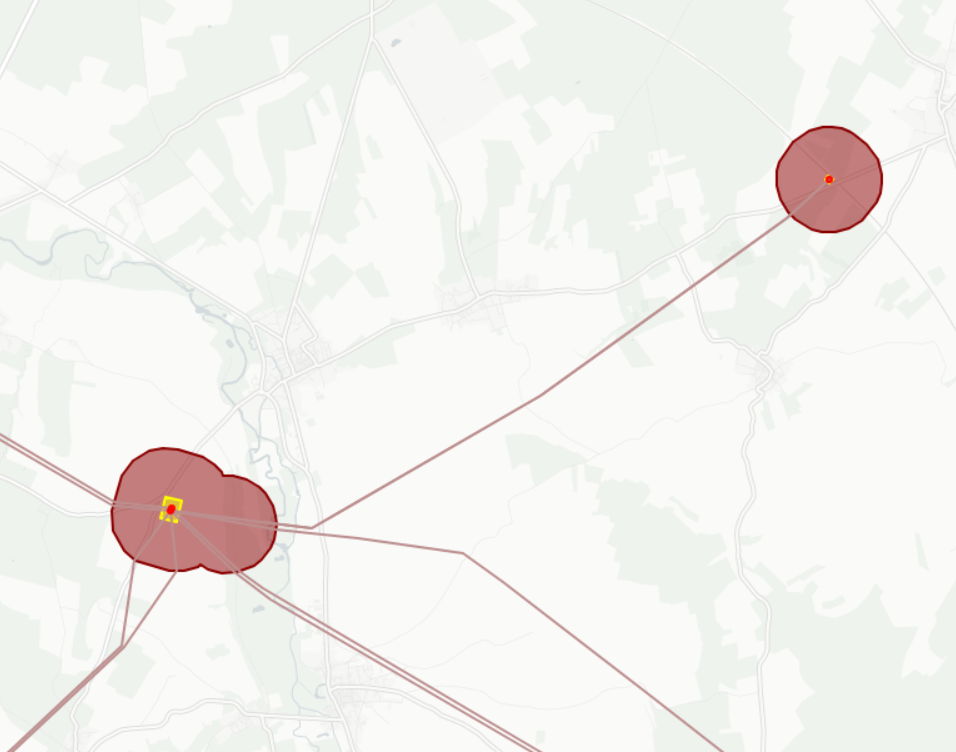
\includegraphics[width=0.65\textwidth]{figures/fig_example_clustering.png}
    \caption{Example for clustering of buses. Taken from the interactive map linked on Zenodo. \cite{xiongPrebuiltElectricityNetwork2024}}
    \label{fig:example_clustering}
\end{figure}

Excerpt of the clustering algorithm as included in the revised manuscript: From each substation polygon and each virtual bus (endpoint of lines/cables), a buffer of 500 meters is created. Substations and virtual buses are then clustered if their buffers overlap (darkred polygon). Then an internal point based on the `Pole of Inaccessibility' \cite{garcia-castellanosPolesInaccessibilityCalculation2007} is determined. With this methodology, we can find a polygon-internal point, even if the polygon is non-convex. If the clustered area contained one or multiple substation(s) from the OSM data, the largest substation sets the geographical coordinates (bright red point) of the clustered substation (yellow polygon). This ensures, that the obtained coordinates are always within the perimeters of an original substation. Polygon internal elements are removed and line/cable endings are modified to exactly end in the determined internal point. Transformers and converters are finally added if necessary and accordingly (see manuscript).


\RC What happens to this model if overpass turbo is not maintained anymore? 

\AR Thank you for your question. We have considered this scenario --- in the event that Overpass turbo is no longer maintained, we can either adapt to another API or use so-called \textit{planet} files, that OpenStreetMap directly provides (\href{https://planet.openstreetmap.org}{https://planet.openstreetmap.org}). These files, provided in .pbf format, are updated every week and contain snapshots of the entire OSM database. The PyPSA-Earth model is using these files via their developed \textit{earth-osm} Python library (\href{https://github.com/pypsa-meets-earth/earth-osm}{https://github.com/pypsa-meets-earth/earth-osm}). Per default, we have deliberately chosen not to use \textit{planet} files in our implementation, as they are very large and require a lot of computational resources and time to process. Electricity-related layers only make up a small fraction of the entire OSM database, this is why we use Overpass Turbo to extract only the relevant data. Further, we would like to highlight that Overpass turbo is a well-established and widely used tool, and we are confident that suitable alternatives would be available in such a scenario. If needed, users can even decide to create their own OSM database mirror and Overpass turbo client if they wish, as the OSM wiki describes (\href{https://wiki.openstreetmap.org/wiki/Overpass_API/Installation}{https://wiki.openstreetmap.org/wiki/Overpass\_API/Installation}).

Lastly, all released prebuilt datasets on Zenodo \cite{xiongPrebuiltElectricityNetwork2024} remain valid and can always be used for modelling purposes, independent of the availability of Overpass turbo. 

\RC Do you also search for the tag \textit{station}, \textit{sub\_station} and the like? some substation in OSM are not well tagged (i.e. do not all have \textit{substation} as tag). 

\AR This is indeed a good idea. We have double-checked this and also queried for variations like \textit{station} and \textit{sub\_station}, however no data was found for the high-voltage grid in the European region. OSM already does a great job in pointing towards well established keys and values such as `power=substation' (\href{https://wiki.openstreetmap.org/wiki/Key:substation}{https://wiki.openstreetmap.org/wiki/Key:substation}) or `power=line' (\href{https://wiki.openstreetmap.org/wiki/Key:power}{https://wiki.openstreetmap.org/wiki/Key:power}). For all of these keys and values, wiki entries exist that point a user to their correct usage. When editing or adding data, contributors are encouraged to follow these guidelines. This is also supported through the OSM web editor, which suggests keys via appearing dropdown menus when typing in the key field.

\RC Did you compare the relations data and the cable/line data representation for DC lines? The same question for AC lines.

\AR We have compared the relations and cables/lines data representation for DC lines. Given the limited number of commissioned DC lines/cables (<40 as of 2024), we have checked every project, individually. Note that ways are members/subsets of relations and all commissioned DC lines/cables represented in ways are contained in relations. As such, we consider the data for DC lines/cables as complete for the European region. For AC cables/lines, we have also compared ways against the relations. Here, the situation is much more complex and heterogeneous, as the number of AC lines is higher by a multitude of dimensions. For example, for countries like Germany and France, we observe that the majority of ways are mapped as members of relations. But this is by far not the case for all remaining countries in Europe. To harness highest data quality available, we have added another step in the data importing and cleaning process following your suggestion. We now query for relations both for AC and DC lines/cables using `relation[route=power]'. Every relation contains the OSM identifiers of all member ways. In a second step we import and clean all those relations that have complete data (i.e., voltage, singular linestrings as geometries, number of circuits). Relational data is then preferred over ways, whenever available. To avoid for duplicates in the representation of a line/cable, all members of relations imported are removed from the set of way, respectively. The manuscript has been updated to reflect this major improvement in the data cleaning process.

\RC There are small typos in the text, which should be corrected. Best regards

\AR Thank you for pointing this out. We have carefully reviewed the manuscript and corrected all typos and minor errors to the best of our knowledge. We appreciate your attention to detail and your feedback.

\section*{Reviewer \#2}

\RC The paper presents a description of several csv datafiles that enable construction of the European high-voltage grid for voltages above 200 kV and a method for obtaining these.

\RC The data is derived from open-street maps and presents new annotations compared to the primary sources via a cleaning procedure and attachment of electrical parameters. As such, the data becomes usable for studies such as energy system modelling, or mere electric power system studies.

\RC The aim of the dataset is to have an openly availably and up-to-date set of lines of the electric power system. Therefore, an automated extraction and cleaning method for data obtained from Open Street Maps is proposed by the authors. The quality of the dataset therefore depends on the Open Street Map contributions. Several heuristics are used to clean the data obtained from Open Street Maps, which are methodologically sound. One of the main assumptions is the use of “standard” transmission line types with associated impedances and nominal powers. With the advent of new transmission line types (e.g., high-temperature low-sag conductors), such an approach may not be suitable for future updates and may require updates to the method.

\AR Thank you for your detailed review and valuable comments. We appreciate your recognition of the potential of our dataset for energy system modelling and electric power system studies. You have raised a valid point regarding the use of standard transmission line types, especially with regards to new transmission line types like high-temperature low-sag conductors. We are exchanging with OSM contributors on how we can track and include this information in OSM sustainably. One solution to this could be to introduce additional keys that allow for the tagging of different line types (or even technical parameters like resistance, impedance, susceptance, nominal current), directly. Some of this data could be transferred from official information provided by institutions like the Joint Allocation Office (JAO), see \cite{jaoStaticGridModel2023}.

\RC The technical quality of the dataset is supported in two ways: (i) through comparison against official statistics from ENTSO-E on European transmission grid line lengths and against data obtained from a German TSO, (ii) through a comparison of an optimization outcome against a benchmark system. 

\RC The first method supports the technical quality of the dataset and proves that the method of retrieving data (using Open Street Maps) can be more reliable than other data sources. 

\RC The first conclusion of the second method, that \textit{both grids adequately represent reality} cannot be stated as such as (i) a future scenario is being evaluated, and (ii) none of both grids represents reality. The reviewer therefore suggests removing this statement. Furthermore, the reviewer suggests to provide more information of the benchmarking case (e.g., the techno-economic assumptions projected for the year 2030), as these are not described. It is not possible to determine in how much the outcomes of this validation case study depend on these assumptions, e.g., whether other assumptions would lead to larger deviations. Could the authors clarify this? 

\AR We appreciate your feedback and your raised question. We agree with you that we cannot make the statement that `both grids adequately represent reality' as we do not have official grid data which are only known to the transmission system operators. As such, we have removed this part of the sentence following your suggestion.

We agree that the model results generally depend on the techno-economic assumption. Note that we have kept every parameter constant in both runs, except for the underlying high-voltage grid. We have run additional typical runs with varying techno-economic assumptions that still show similar results. Following your remarks, we now refer to version 0.9.2 the underlying technology cost assumptions for 2030 (\href{https://zenodo.org/records/13617294}{https://zenodo.org/records/13617294}) \cite{lisazeyenPyPSATechnologydataV0922024} in the manuscript. This enables the reader to get a more transparent view on the potential impact of these assumptions on the validation results.

\RC I am a bit surprised by the statement on the data repository itself: 
\begin{quote}
    The authors of this dataset do not claim correctness, completeness, or any other form of guarantee regarding the information presented.
\end{quote}
Although I understand the reasoning behind this statement, this actually undermines the validation of the dataset provided in this article, and conflicts with the statement that \textit{the grids adequately represents reality}.

\AR We appreciate your feedback and agree with your point. We have removed the statement from the data repository. We are confident in the quality of the dataset and the validation methods we have used. 

\RC The descriptions of the data files in the proposed article is minimal, mainly in that the authors claim that csv files are provided. The authors could provide a more-in depth description of (i) the meaning of the separate data files on the repository, (ii) the structure of each data file, (iii) the size of the data file.

\AR Thank you for your suggestion. We have added detailed descriptions on the meaning of data files, their structure, properties and units, and their file size. Please also see our \hyperref[ac:datarecords]{previous response} (page \pageref{ac:datarecords}). 

\RC As the description of the data file is minimal, it is not possible to verify whether the data files submitted to the repository are complete. First, a discrepancy between the description of the datafiles (e.g., 400 kV is mapped onto 380 kV) was noted, as 400 kV is still included in the \textit{voltage} column of buses.csv. Could the authors please verify this? Second, when verifying e.g., \textit{lines.csv}, it is not possible to find, e.g., electrical parameters such as nominal current or impedance. Could the authors include an improved description of this data in the article?

\AR Thank you for your remarks and questions. We have added detailed descriptions on the meaning of data files, their structure, properties and units, and their file size. Please also see our \hyperref[ac:datarecords]{previous response} (page \pageref{ac:datarecords}). With regard to your question, we need to clarify on what we originally meant in the manuscript. Using the examples of 380 kV and 400 kV voltage levels. Both voltage levels are commonly used for operating transmission grid assets, e.g. 400 kV in Denmark \cite{akhmatovNovelHarmonicDistortion2023} and 380 kV in Germany \cite{bnetzaBestaetigungNetzentwicklungsplanStrom2024} (\href{https://www.entsoe.eu/data/map}{https://www.entsoe.eu/data/map}). When we map pandapower's \cite{thurnerPandapowerOpenSourcePython2018} and PyPSA's \cite{brownPyPSAPythonPower2018} standard linetypes toe the respective lines, we use the closest voltage level available in the dataset. In the case of 380 kV and 400 kV, both are mapped to the `Al/St 240/40 4-bundle 380.0' line type \cite{brownPyPSAPythonPower2018}. Hence, they inherit the same underlying electrical parameters, such as resistance and impedance per km, as well as susceptance and nominal current. However, as they are operated at different voltage levels, as calculating the nominal apparent power includes the multiplication with the voltage level, the nominal apparent power is different for the two voltage levels. The line type column including all electric parameters are now also included in the updated dataset on Zenodo, so this should be more clear now.\cite{xiongPrebuiltElectricityNetwork2024}. We have also made this more clear in the revised manuscript to avoid any confusion.

\bibliography{references.bib}

\end{document}
